\documentclass[11pt]{beamer}
\usetheme{Warsaw}
\usepackage[utf8]{inputenc}
%\usepackage[magyar]{babel}
\usepackage[T1]{fontenc}
\usepackage{amsmath}
\usepackage{amsfonts}
\usepackage{amssymb}
\usepackage{graphicx}
\usepackage{xurl}
\usepackage{multimedia}
\usepackage{xurl}
\author{Bendegúz Borkovits T7UR9P}
\title{Geant4 presentation 2}
%\setbeamercovered{transparent} 
%\setbeamertemplate{navigation symbols}{} 
%\logo{} 
\institute{Scientific Modeling Computer Laboratory} 
\date{March 2022} 
%\subject{} 
\begin{document}


\begin{frame}
\titlepage
\end{frame}

\begin{frame}{Schedule}
\begin{center}
\begin{enumerate}
    \item Last time:
    \begin{itemize}
        \item Installation
        \item Testing
    \end{itemize}
    \item Current development:
    \begin{itemize}
        \item Getting to know the software
        \item Run predefined settings
        \item Change detector geometry
        \item Check the output format
        \item Reproduce figures
    \end{itemize}
\end{enumerate}
\end{center}
\end{frame}

\begin{frame}{Creating a Geant4 project}
    \begin{enumerate}
        \item Create a run manager (contains main function),
        \item define detector construction,
        \item create an action runner,
        \item create a particle generator,
        \item define the physics list.
    \end{enumerate}
\end{frame}

\begin{frame}{Creating a Geant4 project}
    \begin{block}{Run manager}
    Contains main function of the simulation and the execution commands.
    \end{block}
    \begin{block}{Detector construction}
    Contains
    \begin{itemize}
        \item geometry of mother volume,
        \item geometry of detector,
        \item detector material and its properties,
        \item refractive index of detector material.
    \end{itemize}
    \end{block}

    \begin{block}{Action runner}
    Runs particle generating and computes the results.
    \end{block}
\end{frame}

\begin{frame}{Creating a Geant4 project}
    \begin{block}{Particle generator}
    Defines
    \begin{itemize}
        \item particle type,
        \item particle position within the volume,
        \item direction of its momentum,
        \item type of particle generator.
    \end{itemize}
    \end{block}
    
    \begin{block}{Physics list}
    Registers
    \begin{itemize}
        \item physics of the environment,
        \item physics of the detector,
        \item physics to allow for extra particles.
    \end{itemize}
    \end{block}
\end{frame}

\begin{frame}{Built-in libraries}
\begin{columns}
\begin{column}{0.4\textwidth}
    \begin{itemize}
        \item G4RunManager
        \item G4UImanager
        \item G4VisManager
        \item G4VisExecutive
        \item G4UIExecutive
        \item G4ParticleGun
        \item G4LogicalVolume
        \item G4PVPlacement
        \item G4NistManager
    \end{itemize}
\end{column}

\begin{column}{0.6\textwidth}
    \begin{itemize}
        \item G4VUserActionInitialization
        \item G4VUserPrimaryGeneratorAction
        \item G4VUserDetectorConstruction
        \item G4VModularPhysicsList
        \item G4EmStandardPhysics
        \item G4OpticalPhysics
        \item G4VPhysicalVolume
        \item G4SystemOfUnits
        \item G4Box
    \end{itemize}
\end{column}
\end{columns}
\end{frame}

\begin{frame}{Parameters of simulation}
    \begin{block}{Detector construction}
    \begin{itemize}
        \item Aerogel = Silicon + water + carbon
        \item Mother volume is a box (0.5 m, 0.5 m, 0.5 m,)
        \item Detector is a box (0.4 m, 0.4 m, 0.01 m)
    \end{itemize}
    \end{block}
    
    \begin{block}{Particles}
    \begin{itemize}
        \item Particle gun fires one particle.
        \item Proton type.
        \item Momentum is Z-directional and is 100 GeV.
    \end{itemize}
    \end{block}
    
    \begin{block}{Physics}
    \begin{itemize}
        \item Electromagnetic inetraction.
        \item Optical photons. (Not showing, further investigation required.)
    \end{itemize}
    \end{block}
    
    Where is the output?
    
\end{frame}

\begin{frame}{The plan is always flawless}
    \begin{alertblock}{Casualties of war}
    \begin{enumerate}
        \item WSL + Xming do not sync
        \item VirtualBox current version is buggy
        \item VirtualBox older version forgets ISO file
        \item Virtual Ubuntu is dead
        \item Admin issue prevents dual boot
    \end{enumerate}
    \end{alertblock}
    
    \begin{block}{Solution (coming soon)}
    Server machine from the university.
    \end{block}
    \centering
    
\includegraphics[scale = 0.08]{mordor.jpg}
\end{frame}

\begin{frame}{Visualization}
\begin{figure}
    \centering
    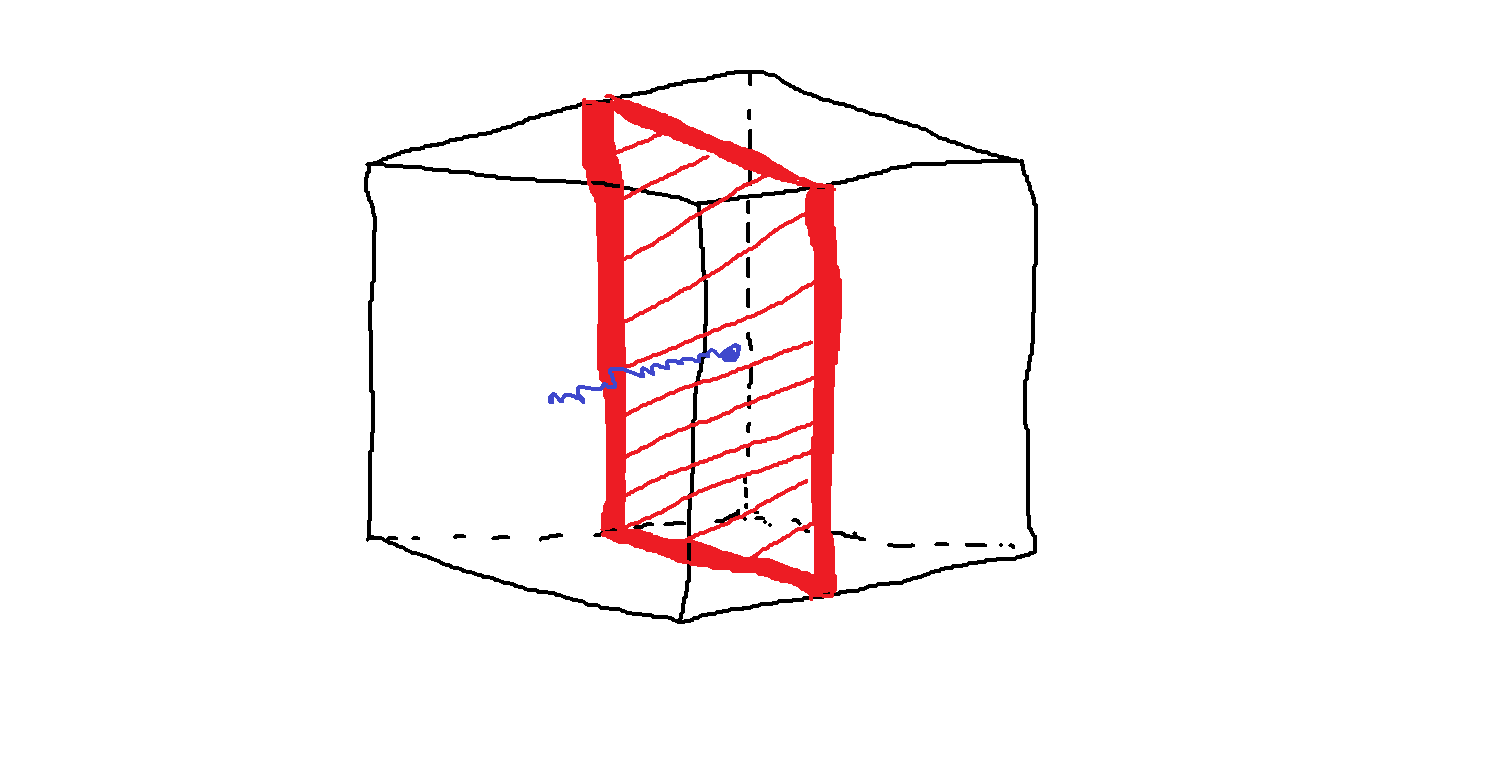
\includegraphics[width = \textwidth]{kreativitas.png}
    The detector and its mother volume. The blue line indicates the trajectory of the proton and the red field is the detector volume.
    \label{fig:my_label}
\end{figure}
    
\end{frame}






\end{document}
